\section{Results}
\label{sec:results}

This section reports the measurements in the order of the research questions. All values are medians or means of the replicates indicated, computed from the stored run folders, and the estimators follow Section~\ref{sec:estimators}. Phase~1 results use the synchronous runtime unless stated otherwise. Phase~2 is the only source of asynchronous and hybrid results, so Phase~2 numbers are not pooled with Phase~1.

\subsection{Model agreement}
\label{sec:model_agree}

Figure~\ref{fig:model} overlays the analytical root quantile on the measured P99.9 for four representative shapes, one per family: chain of depth eight, scatter-gather with fan-out four at depth three, the diamond of width eight at depth five, and the DeathStar social sub-graph. Table~\ref{tab:model} gives the ratio of measured to predicted P99.9 at every stable level of every Phase~1 shape. Across the 60 shape-level pairs that meet the stability criterion, the ratio has a median of $0.62$ and an interquartile range of $0.50$ to $0.70$. The model therefore over-predicts the tail at stable loads by about $1.6$ times at the median.

\begin{figure}[t]
  \centering
  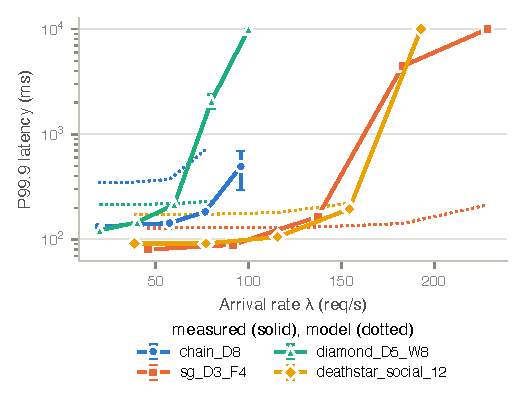
\includegraphics[width=\columnwidth]{fig02.pdf}
  \caption{Measured P99.9 latency against offered rate for four representative shapes, one per call-graph family: chain depth eight, scatter-gather with fan-out four at depth three, diamond with width eight at depth five, and the DeathStar social sub-graph. Solid lines show the mean over replicates with the replicate range as error bars. Dotted lines show the analytical root quantile.}
  \label{fig:model}
\end{figure}

\begin{table}[t]
\centering
\footnotesize
\setlength{\tabcolsep}{3pt}
\caption{Measured P99.9 divided by the analytical root quantile at each stable Phase 1 load level, per shape. Values below one mean that the model over-predicts.}
\label{tab:model}
\resizebox{\linewidth}{!}{%
\begin{tabular}{lllll}
\toprule
\textbf{Shape} & \textbf{$\lvert V\rvert$} & \textbf{Stable levels} & \textbf{Median ratio} & \textbf{Range} \\
\midrule
chain\_D2 & 2 & 4 & 0.67 & 0.62--0.69 \\
chain\_D4 & 4 & 4 & 0.48 & 0.48--0.50 \\
chain\_D6 & 6 & 4 & 0.43 & 0.38--0.68 \\
chain\_D8 & 8 & 4 & 0.38 & 0.26--0.39 \\
deathstar\_hotel\_8 & 8 & 3 & 0.61 & 0.60--0.74 \\
deathstar\_social\_12 & 12 & 3 & 0.53 & 0.53--0.58 \\
diamond\_D3\_W4 & 7 & 3 & 0.65 & 0.64--0.98 \\
diamond\_D3\_W8 & 11 & 4 & 1.08 & 0.67--3.69 \\
diamond\_D5\_W4 & 15 & 3 & 0.60 & 0.50--0.70 \\
diamond\_D5\_W8 & 27 & 3 & 0.67 & 0.57--0.98 \\
diamond\_D6\_W4 & 19 & 3 & 0.49 & 0.45--0.65 \\
diamond\_D7\_W4 & 23 & 3 & 0.46 & 0.44--0.58 \\
sg\_D2\_F2 & 3 & 4 & 0.69 & 0.65--1.30 \\
sg\_D2\_F4 & 5 & 3 & 0.74 & 0.72--0.77 \\
sg\_D2\_F8 & 9 & 3 & 0.74 & 0.72--0.97 \\
sg\_D3\_F2 & 7 & 3 & 0.60 & 0.59--0.64 \\
sg\_D3\_F4 & 21 & 3 & 0.69 & 0.62--1.25 \\
sg\_D4\_F2 & 15 & 3 & 0.57 & 0.54--0.62 \\
\bottomrule
\end{tabular}%
}
\end{table}


The error is not uniform across load. It reverses near saturation. At the highest stable level, the measured P99.9 exceeded the M0 prediction for three shapes: the width-eight in-cast by a factor of $3.69$, the scatter-gather graph with fan-out two at depth two by $1.30$, and the scatter-gather graph with fan-out four at depth three by $1.25$. The reversal occurs at the top stable level, where queueing is largest.

The two diagnostics of Section~\ref{sec:model_diag} separate the two kinds of error. Replacing only the root's shape parameter by the path SCV, $c_s^2/L$, moves the chains to a median of $0.91$ to $0.96$, which is the expected effect if the chain error comes from the root's fixed shape. The overall median rises to $1.04$ (interquartile range $0.98$ to $1.19$), but only because errors of opposite sign cancel across families. The same replacement pushes the fan-out ratios further above one. At the highest stable level of the width-eight in-cast it gives $6.30$, and the median over the four stable levels of that shape is $1.85$. The fan-out error therefore does not come from the root's shape parameter.

The order-statistic extension M1 was tested as a second route to the fan-out error. Over the same 60 pairs its median is $1.10$ (interquartile range $1.00$ to $1.19$), against $1.04$ for the path diagnostic. Table~\ref{tab:m1_summary} gives the family medians and the highest-level ratios for the three shapes discussed above. The highest-level ratio for the width-eight in-cast rises from $3.69$ under M0 to $6.89$ under M1, and for the scatter-gather graph with fan-out four at depth three it rises from $1.25$ to $2.02$. For the scatter-gather graph with fan-out two at depth two it falls from $1.30$ to $0.97$. M1 therefore does not close the fan-out gap, and it makes the in-cast worse. We report it as an exploratory negative result. The mechanism behind the fan-out error is not identified by these diagnostics. The omitted terms of the model appear to be its source, but the campaign does not isolate them.

\begin{table}[t]
\centering
\footnotesize
\caption{Analytical diagnostics against measured P99.9 at the stable load levels. Each entry is the ratio of measured to predicted P99.9 (values below one mean over-prediction). Upper rows summarize all 60 shape-level pairs by call-graph family; lower rows give the highest stable level of the three shapes discussed in the text.}
\label{tab:m1_summary}
\resizebox{\linewidth}{!}{%
\begin{tabular}{@{}lrrrr@{}}
\toprule
Group & Pairs & M0 median & Path-SCV median & M1 median \\
\midrule
chain & 16 & 0.48 & 0.92 & 0.95 \\
deathstar & 6 & 0.59 & 1.04 & 1.09 \\
diamond & 19 & 0.65 & 1.23 & 1.23 \\
sg & 19 & 0.69 & 1.06 & 1.11 \\
All pairs & 60 & 0.62 & 1.04 & 1.10 \\
\midrule
Shape (highest stable level) & Rate (req/s) & M0 & Path-SCV & M1 \\
\midrule
diamond\_D3\_W8 & 80.0 & 3.69 & 6.30 & 6.89 \\
sg\_D3\_F4 & 137.1 & 1.25 & 2.13 & 2.02 \\
sg\_D2\_F2 & 312.2 & 1.30 & 1.87 & 0.97 \\
\bottomrule
\end{tabular}%
}
\end{table}


\subsection{RQ1: Tail amplification and depth}
\label{sec:rq1}

Table~\ref{tab:amplification} reports the amplification factors and the saturation horizons for the 18 Phase~1 shapes. For 17 of the 18 shapes, $\Gamma_{\mathrm{crit}}$ lies between $2.84$ and $8.14$ at the highest stable load. The width-eight in-cast of depth three (\texttt{diamond\_D3\_W8}) reaches $20.53$, which is the largest value in the campaign. At its highest stable level of $80$\,req/s its utilization is $0.88$, and its P99.9 is $504.8\,\mathrm{ms}$ against $86.1\,\mathrm{ms}$ at the lowest level. Queueing near saturation is the likely cause of this amplification.

\begin{table*}[t]
\centering
\footnotesize
\setlength{\tabcolsep}{3pt}
\caption{Phase 1 shapes (synchronous runtime): amplification factors at the highest stable load, and saturation horizons $\Theta^*$ (req/s), each with the two load levels that enclose it in brackets.}
\label{tab:amplification}
\resizebox{\linewidth}{!}{%
\begin{tabular}{llllll}
\toprule
\textbf{Shape} & \textbf{Runtime} & \textbf{$\lvert V\rvert$} & \textbf{$\Gamma_{\mathrm{crit}}$ (P99.9)} & \textbf{$\Gamma_{\mathrm{load}}$ (P99.9)} & \textbf{$\Theta^*$} \\
\midrule
chain\_D2 & sync & 2 & 4.26 & 1.22 & 312.2 [234.1, 312.2] \\
chain\_D4 & sync & 4 & 3.28 & 1.28 & 154.2 [115.7, 154.2] \\
chain\_D6 & sync & 6 & 3.01 & 0.82 & 102.4 [76.8, 102.4] \\
chain\_D8 & sync & 8 & 2.84 & 1.38 & 76.6 [57.5, 76.6] \\
deathstar\_hotel\_8 & sync & 8 & 4.03 & 1.28 & 154.8 [103.2, 154.8] \\
deathstar\_social\_12 & sync & 12 & 3.20 & 1.15 & 154.2 [115.7, 154.2] \\
diamond\_D3\_W4 & sync & 7 & 5.16 & 1.57 & 120.0 [80.0, 120.0] \\
diamond\_D3\_W8 & sync & 11 & 20.53 & 5.86 & 80.0 [60.0, 80.0] \\
diamond\_D5\_W4 & sync & 15 & 3.86 & 1.25 & 92.3 [61.5, 92.3] \\
diamond\_D5\_W8 & sync & 27 & 5.12 & 1.76 & 60.0 [40.0, 60.0] \\
diamond\_D6\_W4 & sync & 19 & 3.64 & 1.53 & 102.4 [76.8, 102.4] \\
diamond\_D7\_W4 & sync & 23 & 3.22 & 1.39 & 87.7 [65.8, 87.7] \\
sg\_D2\_F2 & sync & 3 & 8.14 & 2.19 & 312.2 [234.1, 312.2] \\
sg\_D2\_F4 & sync & 5 & 4.09 & 1.09 & 312.2 [234.1, 312.2] \\
sg\_D2\_F8 & sync & 9 & 5.47 & 1.39 & 234.1 [156.1, 234.1] \\
sg\_D3\_F2 & sync & 7 & 3.68 & 1.14 & 206.4 [154.8, 206.5] \\
sg\_D3\_F4 & sync & 21 & 6.64 & 2.05 & 137.1 [91.4, 137.1] \\
sg\_D4\_F2 & sync & 15 & 3.34 & 1.19 & 154.2 [115.7, 154.2] \\
\bottomrule
\end{tabular}%
}
\end{table*}


Along chains, $\Gamma_{\mathrm{crit}}$ falls with depth, from $4.26$ at depth two to $2.84$ at depth eight (Figure~\ref{fig:amp}). The fall comes from the normalization, not from a shrinking tail. The implied critical-path median sum grows from $16.6\,\mathrm{ms}$ to $64.5\,\mathrm{ms}$, while the measured P99.9 at the highest stable level grows from $70.7\,\mathrm{ms}$ to $182.8\,\mathrm{ms}$. The P99.9 therefore grows by a factor of $2.6$ while the critical-path median grows by a factor of $3.9$, and that is why the ratio falls. The absolute tail therefore grows with depth; only the normalized factor falls.

The amplification relative to the load baseline, $\Gamma_{\mathrm{load}}$, lies between $0.82$ and $2.19$ for the 17 shapes above, and it is $5.86$ for the width-eight in-cast. Three values fall below one. These are chain depth six under the synchronous runtime ($0.82$), and chain depth eight under the asynchronous and hybrid runtimes ($0.96$ and $0.98$). We read these as noise in the base-level tail rather than as a real decrease in tail latency. At the lowest load of a shape, a run holds only a few thousand measured requests, so its P99.9 rests on a handful of samples. For chain depth six, the base-level P99.9 of $177\,\mathrm{ms}$ exceeds the top stable level's $145\,\mathrm{ms}$.

\begin{figure}[t]
  \centering
  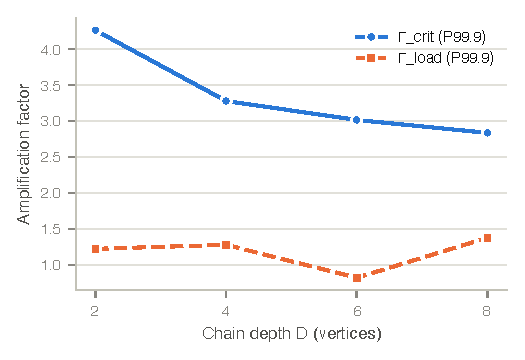
\includegraphics[width=\columnwidth]{fig01.pdf}
  \caption{Amplification factors against chain depth for the four chain shapes at the highest stable load: $\Gamma_{\mathrm{crit}}$ (upper curve) and $\Gamma_{\mathrm{load}}$ (lower curve), both at P99.9.}
  \label{fig:amp}
\end{figure}

The generalized Pareto shape parameter $\xi$ is negative, with a 95\% interval below zero, for 11 of the 18 shapes. Its interval includes zero for five shapes, and it is positive, with an interval above zero, for two scatter-gather graphs. These are the fan-out two graph at depth two ($\xi=0.53$, interval 0.49 to 0.58) and the fan-out four graph at depth three ($\xi=0.09$, interval 0.03 to 0.15). Table~\ref{tab:tails} lists the values, and Figure~\ref{fig:gpd} shows a diagnostic of the fit for the run with the most measured requests. A bounded tail contradicts the heavy-tail premise, so the heavy-tail claim holds only for those two graphs. Their upper bracket levels sit at root utilizations of $0.84$ and $0.76$. The data cannot separate a property of the call graph from queueing close to saturation, because both shapes were measured near the edge of their stable range.

\begin{table*}[t]
\centering
\footnotesize
\setlength{\tabcolsep}{3pt}
\caption{Phase 1 shapes: generalized Pareto tail parameters above the 95th percentile at the highest stable load, with 95\% bootstrap intervals for $\xi$.}
\label{tab:tails}
\resizebox{\linewidth}{!}{%
\begin{tabular}{lllll}
\toprule
\textbf{Shape} & \textbf{Runtime} & \textbf{Excesses} & \textbf{$\xi$ [95\% CI]} & \textbf{$\sigma$ (ms)} \\
\midrule
chain\_D2 & sync & 2501 & -0.04 [-0.08, -0.00] & 7.654 \\
chain\_D4 & sync & 1237 & -0.06 [-0.12, -0.00] & 10.973 \\
chain\_D6 & sync & 818 & 0.01 [-0.07, 0.06] & 12.094 \\
chain\_D8 & sync & 609 & -0.21 [-0.30, -0.16] & 20.940 \\
deathstar\_hotel\_8 & sync & 1237 & -0.11 [-0.16, -0.06] & 9.941 \\
deathstar\_social\_12 & sync & 926 & -0.11 [-0.17, -0.06] & 10.020 \\
diamond\_D3\_W4 & sync & 952 & -0.01 [-0.08, 0.05] & 11.988 \\
diamond\_D3\_W8 & sync & 648 & -0.37 [-0.42, -0.32] & 75.394 \\
diamond\_D5\_W4 & sync & 739 & -0.09 [-0.18, -0.02] & 16.608 \\
diamond\_D5\_W8 & sync & 475 & -0.15 [-0.23, -0.08] & 24.593 \\
diamond\_D6\_W4 & sync & 621 & -0.16 [-0.23, -0.09] & 19.661 \\
diamond\_D7\_W4 & sync & 523 & -0.05 [-0.13, 0.04] & 18.272 \\
sg\_D2\_F2 & sync & 2486 & 0.53 [0.49, 0.58] & 11.963 \\
sg\_D2\_F4 & sync & 1872 & -0.07 [-0.11, -0.03] & 7.569 \\
sg\_D2\_F8 & sync & 1872 & -0.02 [-0.07, 0.02] & 9.379 \\
sg\_D3\_F2 & sync & 1248 & -0.03 [-0.10, 0.02] & 7.479 \\
sg\_D3\_F4 & sync & 1097 & 0.09 [0.03, 0.15] & 17.777 \\
sg\_D4\_F2 & sync & 920 & -0.12 [-0.18, -0.06] & 10.520 \\
\bottomrule
\end{tabular}%
}
\end{table*}


\begin{figure}[t]
  \centering
  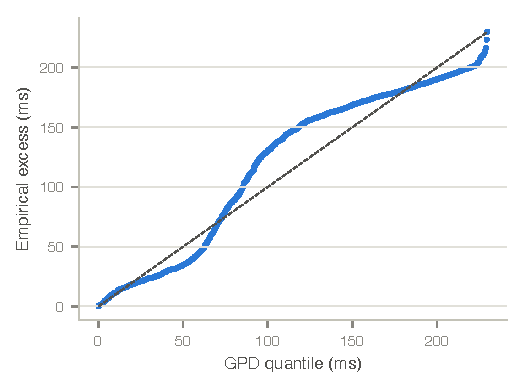
\includegraphics[width=\columnwidth]{fig05.pdf}
  \caption{Empirical excess quantiles against generalized Pareto quantiles for one run, the one with the most measured requests, above its 95th percentile. The dashed line is the identity.}
  \label{fig:gpd}
\end{figure}

\subsection{RQ2: Saturation horizon and CPU utilization}
\label{sec:rq2}

The saturation horizon $\Theta^*$ is reported as the bracket of measured load levels that encloses it, together with the stability fraction described in Section~\ref{sec:estimators}. Figure~\ref{fig:horizon} shows the bracket for every Phase~1 shape. Along chains, the bracket falls from $234$ to $312$\,req/s at depth two to $57$ to $77$\,req/s at depth eight. For the depth-three diamond it falls from $80$ to $120$\,req/s at width four to $60$ to $80$\,req/s at width eight. The ordering matches the model's first two predictions. Deep chains and wide in-casts saturate at lower rates.

The brackets are stable in most shapes. For 16 of the 18 shapes, at least 99.9\% of the bootstrap resamples return the same bracket. The two exceptions are chain depth six, at 78\%, and the diamond of width four and depth five, at 79\%. For six shapes the upper bracket level has root utilization of at least $0.9$, and so lies beyond the stability cutoff: the DeathStar social sub-graph ($0.91$), the diamond with width four at depth six ($0.96$), the diamond with width four at depth seven ($0.93$), the scatter-gather graphs with fan-out four at depth two ($0.92$) and fan-out two at depth three ($0.95$), and the scatter-gather graph with fan-out two at depth four ($0.97$). For these shapes the curvature horizon and the stability cutoff disagree, and we report both.

\begin{figure}[t]
  \centering
  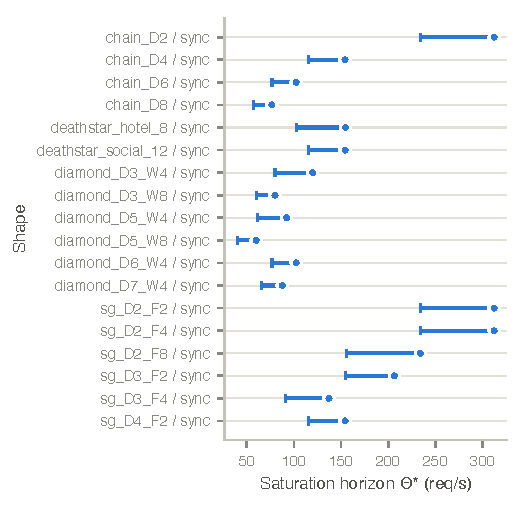
\includegraphics[width=\columnwidth]{fig04.pdf}
  \caption{Saturation horizon $\Theta^*$ for each Phase~1 shape. Each bar spans the bracket of measured load levels that encloses the point estimate, so it is not a confidence interval.}
  \label{fig:horizon}
\end{figure}

The reason the chains saturate at low CPU is visible in the root pool and the host processors. Figure~\ref{fig:poolcpu} plots root pool utilization against the measured CPU utilization of the mesh processes, one point per run. On the four chains, the root pool reaches utilization $0.75$ to $0.79$ at the upper bracket level while the processes use $9.2\%$ to $10.3\%$ of the eight cores (Table~\ref{tab:knee}). Saturation on chains therefore occurs at low CPU, which indicates that the root thread pool binds before the processors do. The pattern weakens for wider graphs. At the upper bracket level the width-eight in-cast reaches utilization $0.88$ at $35\%$ CPU, and the width-four diamond of depth seven reaches $0.93$ at $45\%$ CPU.

\begin{table*}[t]
\centering
\footnotesize
\setlength{\tabcolsep}{3pt}
\caption{Root pool utilization, host CPU, and timeouts at the upper bracket level of each Phase 1 shape. Root utilization above 0.9 lies beyond the stability cutoff.}
\label{tab:knee}
\resizebox{\linewidth}{!}{%
\begin{tabular}{llllll}
\toprule
\textbf{Shape} & \textbf{$\lvert V\rvert$} & \textbf{Level (req/s)} & \textbf{Root utilization} & \textbf{Host CPU (\%)} & \textbf{Timeouts (\%)} \\
\midrule
chain\_D2 & 2 & 312.2 & 0.79 & 9.2 & 0.0 \\
chain\_D4 & 4 & 154.2 & 0.77 & 9.9 & 0.0 \\
chain\_D6 & 6 & 102.4 & 0.76 & 10.1 & 0.0 \\
chain\_D8 & 8 & 76.6 & 0.75 & 10.3 & 0.0 \\
deathstar\_hotel\_8 & 8 & 154.8 & 0.74 & 25.7 & 0.0 \\
deathstar\_social\_12 & 12 & 154.2 & 0.91 & 31.3 & 0.0 \\
diamond\_D3\_W4 & 7 & 120.0 & 0.68 & 25.6 & 0.0 \\
diamond\_D3\_W8 & 11 & 80.0 & 0.88 & 34.7 & 0.0 \\
diamond\_D5\_W4 & 15 & 92.3 & 0.74 & 33.5 & 0.0 \\
diamond\_D5\_W8 & 27 & 60.0 & 0.62 & 44.2 & 0.0 \\
diamond\_D6\_W4 & 19 & 102.4 & 0.96 & 45.1 & 0.0 \\
diamond\_D7\_W4 & 23 & 87.7 & 0.93 & 45.0 & 0.0 \\
sg\_D2\_F2 & 3 & 312.2 & 0.84 & 14.4 & 0.0 \\
sg\_D2\_F4 & 5 & 312.2 & 0.92 & 25.6 & 0.0 \\
sg\_D2\_F8 & 9 & 234.1 & 0.76 & 35.4 & 0.0 \\
sg\_D3\_F2 & 7 & 206.5 & 0.95 & 24.0 & 0.0 \\
sg\_D3\_F4 & 21 & 137.1 & 0.76 & 50.9 & 0.0 \\
sg\_D4\_F2 & 15 & 154.2 & 0.97 & 39.8 & 0.0 \\
\bottomrule
\end{tabular}%
}
\end{table*}


\begin{figure}[t]
  \centering
  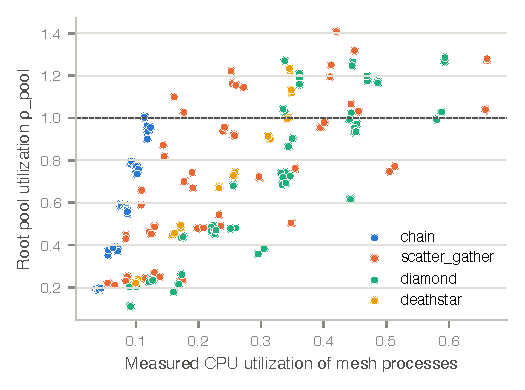
\includegraphics[width=\columnwidth]{fig03.pdf}
  \caption{Root pool utilization against measured CPU utilization of the mesh processes, one point per run. Colours mark the four call-graph families (chain, scatter-gather, diamond, and DeathStar sub-graphs), and the dashed line marks utilization of one.}
  \label{fig:poolcpu}
\end{figure}

\subsection{Runtime comparison and the in-cast mechanism}
\label{sec:runtimes}

Phase~2 compares the three runtimes at the same five offered loads for three shapes, a depth-eight chain, a 21-vertex scatter-gather graph, and a 27-vertex diamond of width eight. Table~\ref{tab:runtimes} gives the median P99.9 at each level across three replicates. The comparison does not depend on the stability criterion, because every runtime is evaluated at the same loads.

On the depth-eight chain, the synchronous runtime is the first to degrade. Its median P99.9 rises from $192.5\,\mathrm{ms}$ at $76.6$\,req/s to the $10\,\mathrm{s}$ timeout ceiling at $115$\,req/s, where $11.7\%$ of requests time out. The asynchronous and hybrid chains stay between $114$ and $135\,\mathrm{ms}$ at every load up to $191.6$\,req/s, with no timeouts, so no saturation horizon appears for them. At 77 and 115\,req/s the three runtimes use similar CPU, between $0.8$ and $1.2$ cores. Above 115\,req/s the synchronous CPU stops rising because its requests fail, whereas the asynchronous and hybrid runtimes continue to rise to about $1.9$ cores at the top load. The CPU comparison therefore reflects which runtime still serves the offered load.

On the 21-vertex scatter-gather graph, the synchronous P99.9 rises from $118\,\mathrm{ms}$ at $137$\,req/s to $4.2\,\mathrm{s}$ at $183$\,req/s. The asynchronous and hybrid runtimes stay between $72$ and $89\,\mathrm{ms}$ up to $137$\,req/s and reach $107$ and $119\,\mathrm{ms}$ at $183$\,req/s. On the 27-vertex diamond, the synchronous runtime times out on $41\%$ of requests at $94$\,req/s, where the asynchronous P99.9 is $406\,\mathrm{ms}$ and the hybrid P99.9 is $2.1\,\mathrm{s}$. The hybrid runtime is slower than the asynchronous one on the in-cast, although the two are similar on the chain and on the scatter-gather graph.

\begin{table*}[t]
\centering
\footnotesize
\setlength{\tabcolsep}{3pt}
\caption{Runtime comparison at the same five loads for three shapes: median P99.9 (ms) across three replicates. Load rows give the offered rate of each level. Asterisks mark levels where more than 1\% of requests timed out.}
\label{tab:runtimes}
\resizebox{\linewidth}{!}{%
\begin{tabular}{lllllll}
\toprule
\textbf{Shape} & \textbf{Runtime / load} & \textbf{L1} & \textbf{L2} & \textbf{L3} & \textbf{L4} & \textbf{L5} \\
\midrule
chain\_D8 & load (req/s) & 38.3 & 76.6 & 115.0 & 153.3 & 191.6 \\
 & sync & 138.6 & 192.5 & 10018.8$^{*}$ & 10018.8$^{*}$ & 10018.8$^{*}$ \\
 & aio & 118.5 & 114.1 & 114.3 & 118.0 & 120.5 \\
 & hybrid & 134.8 & 132.1 & 131.3 & 132.7 & 134.5 \\
sg\_D3\_F4 & load (req/s) & 45.7 & 91.4 & 137.1 & 182.9 & 228.6 \\
 & sync & 81.9 & 85.1 & 117.8 & 4159.5 & 10018.8$^{*}$ \\
 & aio & 76.5 & 72.1 & 76.7 & 106.8 & 219.8 \\
 & hybrid & 82.3 & 81.0 & 88.8 & 119.3 & 229.9 \\
diamond\_D5\_W8 & load (req/s) & 23.4 & 46.8 & 70.2 & 93.7 & 117.1 \\
 & sync & 121.3 & 163.5 & 372.0 & 10018.8$^{*}$ & 10018.8$^{*}$ \\
 & aio & 98.6 & 114.4 & 217.0 & 406.0 & 3479.6 \\
 & hybrid & 114.8 & 137.3 & 338.4 & 2113.5 & 4309.0 \\
\bottomrule
\end{tabular}%
}
\end{table*}


The stored hop records locate the difference at the two shared leaves, each of which receives about eight calls per root request. Across three replicates at $93.7$\,req/s, the median wait for a leaf worker is 25 to 46\,ms under the synchronous and asynchronous runtimes and 1.05 to 1.47\,s under the hybrid runtime. The median local work time at the leaves is 9 to 10\,ms under the first two runtimes and 29 to 34\,ms under the hybrid runtime. The upstream pool wait stays near 1\,ms under the asynchronous and hybrid runtimes, and near 0.35\,ms under the synchronous runtime. The queue therefore forms at the shared leaves, not upstream. The upstream hop time includes the leaf wait, so the upstream latency is large under the hybrid runtime even though the upstream pool is not congested.

The local work at the leaves is dilated about threefold under the hybrid runtime, and the dilation coincides with the leaf queue. The data establish the dilation and the wait, but they do not decompose the wait into its causes. Our working hypothesis is that CPython's global interpreter lock and the wakeup of worker threads from the event loop are responsible. In the hybrid runtime, the event-loop thread deserializes incoming frames and dispatches callbacks while eight pool workers run the busy-loop share of the local work, and every leaf invocation then pays a cross-thread handoff. That hypothesis is consistent with the measurements and with the default GIL switch interval of $5\,\mathrm{ms}$. It has not been tested by an experiment that removes one of its components, so we report it as a mechanism to test, not as a result.

The runtimes are also limited by different resources. Under the asynchronous runtime, the event loop carries the local work, so the loop is busy even when no thread is held. For that reason the root utilization reported for the asynchronous and hybrid runtimes is a holding-time measure, computed from the root's hop holding time in the same way as Eq.~\eqref{eq:rho}, and it is not a measure of pool occupancy. Values above one in the high-load rows of Phase~2 therefore do not indicate a queue at a bounded pool.

\subsection{RQ3: Serialization and sidecar tax}
\label{sec:rq3}

Table~\ref{tab:tax} and Figure~\ref{fig:tax} separate the two costs of the sidecar emulation. Serialization, the protocol-buffer encode and decode time, accounts for $0.20\%$ to $0.76\%$ of CPU per request, and its share rises with payload size. Protocol-buffer accelerators target workloads in which serialization dominates~\cite{karandikar2021protoacc}, and these small payloads are not such a workload. The sidecar emulation accounts for $23\%$ to $32\%$ of CPU, and its share changes by at most $3.5$ percentage points across payloads at each depth. The median per-hop edge overhead, which is the caller's wall time minus the callee's own hop time, lies between $1.8$ and $3.4\,\mathrm{ms}$. At 30\,req/s, the P99 latency grows with depth, from $42$ to $50\,\mathrm{ms}$ at depth two, to $72$ to $79\,\mathrm{ms}$ at depth four, and to $126$ to $133\,\mathrm{ms}$ at depth eight. It shows no systematic change with payload.

The sidecar's cost is therefore a large share of CPU and a fixed per-hop latency. The proxy is a bytes-passthrough emulation, not Envoy, so these numbers describe the mechanism and not a production deployment. A production proxy also applies routing and telemetry filters that the emulation omits, so the figures should be remeasured on a production proxy before they are used for capacity planning.

\begin{table*}[t]
\centering
\footnotesize
\setlength{\tabcolsep}{3pt}
\caption{Medians across five replicates per cell at 30\,req/s: serialization and sidecar shares of CPU per request, median per-hop edge overhead, and P99 latency.}
\label{tab:tax}
\resizebox{\linewidth}{!}{%
\begin{tabular}{llllll}
\toprule
\textbf{Depth} & \textbf{Payload (B)} & \textbf{Serialization} & \textbf{Sidecar} & \textbf{Edge overhead (ms)} & \textbf{P99 (ms)} \\
\midrule
2 & 64 & 0.30\% & 26.1\% & 3.13 & 47.6 \\
2 & 1024 & 0.37\% & 26.1\% & 3.17 & 49.5 \\
2 & 4096 & 0.31\% & 22.9\% & 1.89 & 42.4 \\
2 & 16384 & 0.45\% & 22.7\% & 1.94 & 46.2 \\
2 & 65536 & 0.66\% & 26.2\% & 3.40 & 48.4 \\
4 & 64 & 0.20\% & 28.5\% & 1.78 & 73.8 \\
4 & 1024 & 0.32\% & 31.9\% & 2.98 & 78.1 \\
4 & 4096 & 0.33\% & 32.0\% & 2.99 & 78.6 \\
4 & 16384 & 0.52\% & 31.0\% & 2.59 & 72.3 \\
4 & 65536 & 0.76\% & 30.3\% & 2.60 & 77.8 \\
8 & 64 & 0.26\% & 31.0\% & 1.84 & 131.6 \\
8 & 1024 & 0.28\% & 31.0\% & 1.96 & 131.5 \\
8 & 4096 & 0.32\% & 30.9\% & 1.94 & 132.5 \\
8 & 16384 & 0.49\% & 30.6\% & 1.82 & 126.3 \\
8 & 65536 & 0.76\% & 30.0\% & 1.85 & 132.0 \\
\bottomrule
\end{tabular}%
}
\end{table*}


\begin{figure*}[t]
  \centering
  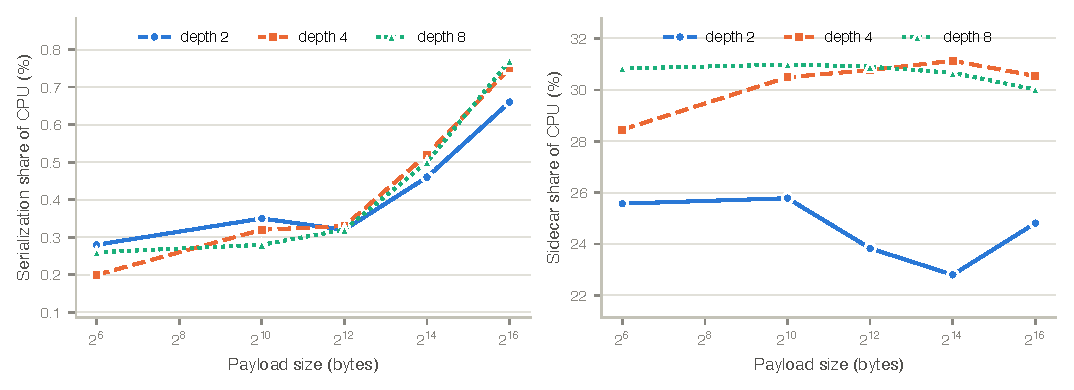
\includegraphics[width=\textwidth]{fig07.pdf}
  \caption{Serialization share of CPU (left) and sidecar share of CPU (right) against payload size, with one series per call-graph depth.}
  \label{fig:tax}
\end{figure*}

\subsection{RQ4: Tracing overhead}
\label{sec:tracing}

Phase~4 compares each traced configuration with the rate-zero baseline at the same load (Table~\ref{tab:tracing}). The medians across replicates are used throughout, because one baseline replicate at the high load reached $385\,\mathrm{ms}$ at P99.9 while the other five lay between $79$ and $85\,\mathrm{ms}$, and the mean would be dominated by that run. Each traced configuration has three replicates, so the comparisons are small.

At the low load of $38.6$\,req/s, all eight traced configurations read $1.2$ to $7.0\,\mathrm{ms}$ lower at P99 than the baseline. A tracing system cannot reduce latency, so this result is a confound. The baseline ran under higher host background, with a median of $0.66$ cores against $0.14$ to $0.90$ cores for the traced configurations. We therefore do not interpret the low-load differences as a property of tracing.

At the high load of $115.7$\,req/s, just below saturation on the four-vertex chain, the rate-zero baseline shows a median P99 of $67.5\,\mathrm{ms}$ and a median P99.9 of $82.3\,\mathrm{ms}$. The six configurations with sampling rate $S\ge0.25$ move P99 into the $71.8$ to $78.1\,\mathrm{ms}$ range, a shift of $+4.3$ to $+10.6\,\mathrm{ms}$, and P99.9 into the $85.5$ to $95.1\,\mathrm{ms}$ range, a shift of $+3.2$ to $+12.8\,\mathrm{ms}$. The baseline at this load ran under higher background CPU, $0.93$ cores against $0.11$ to $0.41$ cores for these traced cells. Higher background load raises the queueing tail, so the baseline's latency is inflated relative to a background-free baseline. Under that monotone assumption the observed difference is biased toward zero, and it is a conservative lower bound on the tracing effect. The bound depends on that assumption, and we state it as such.

Pooling all $6\times3=18$ high-load runs with $S\ge0.25$ gives a non-parametric bootstrap median overhead of $+5.50\,\mathrm{ms}$ at P99 (95\% interval $[+2.88, +7.17]\,\mathrm{ms}$, or $+8.2\%$) and $+5.86\,\mathrm{ms}$ at P99.9 ($+7.1\%$). All six configurations show a positive shift at both quantiles, which gives an exact two-sided sign test with $p=0.03125$. This test is over six configurations, each with three replicates, so the evidence is limited, and the effect is reported as suggestive. The exporter mode does not produce a consistent difference. At the high load, the batch and synchronous exporters differ by $0.7$ to $4.7\,\mathrm{ms}$ at P99 across the sampling rates with $S\ge0.25$, and the sign of the difference changes with the rate. We do not attribute the overhead to span serialization or to span creation, because the experiment does not separate those costs.

\begin{table*}[t]
\centering
\footnotesize
\setlength{\tabcolsep}{3pt}
\caption{Tracing overhead on a four-vertex chain at two loads, as medians across replicates (three per traced configuration, six for the rate-zero baseline). Deltas are traced minus the baseline at the same load. Background is the median host background of the runs.}
\label{tab:tracing}
\resizebox{\linewidth}{!}{%
\begin{tabular}{llllllll}
\toprule
\textbf{Exporter} & \textbf{Sampling} & \textbf{Load (req/s)} & \textbf{P99 (ms)} & \textbf{$\Delta$P99 (ms)} & \textbf{P99.9 (ms)} & \textbf{$\Delta$P99.9 (ms)} & \textbf{Background (cores)} \\
\midrule
none & 0.00 & 38.6 & 75.6 & +0.0 & 89.8 & +0.0 & 0.66 \\
none & 0.00 & 115.7 & 67.5 & +0.0 & 82.3 & +0.0 & 0.93 \\
batch & 0.10 & 38.6 & 72.8 & -2.7 & 85.6 & -4.2 & 0.18 \\
batch & 0.10 & 115.7 & 67.5 & +0.0 & 80.6 & -1.7 & 0.46 \\
sync & 0.10 & 38.6 & 74.4 & -1.2 & 91.1 & +1.3 & 0.84 \\
sync & 0.10 & 115.7 & 66.9 & -0.6 & 80.2 & -2.1 & 0.76 \\
batch & 0.25 & 38.6 & 73.6 & -2.0 & 85.5 & -4.3 & 0.14 \\
batch & 0.25 & 115.7 & 72.4 & +4.9 & 85.5 & +3.2 & 0.11 \\
sync & 0.25 & 38.6 & 72.4 & -3.2 & 88.3 & -1.5 & 0.15 \\
sync & 0.25 & 115.7 & 73.5 & +6.0 & 89.4 & +7.1 & 0.11 \\
batch & 0.50 & 38.6 & 70.1 & -5.5 & 80.8 & -9.0 & 0.60 \\
batch & 0.50 & 115.7 & 72.5 & +5.0 & 86.1 & +3.8 & 0.21 \\
sync & 0.50 & 38.6 & 71.6 & -4.0 & 84.6 & -5.2 & 0.15 \\
sync & 0.50 & 115.7 & 71.8 & +4.3 & 88.4 & +6.1 & 0.13 \\
batch & 1.00 & 38.6 & 68.5 & -7.0 & 81.0 & -8.8 & 0.90 \\
batch & 1.00 & 115.7 & 78.1 & +10.6 & 95.1 & +12.8 & 0.41 \\
sync & 1.00 & 38.6 & 69.2 & -6.4 & 80.4 & -9.3 & 0.88 \\
sync & 1.00 & 115.7 & 73.3 & +5.9 & 92.2 & +9.9 & 0.27 \\
\bottomrule
\end{tabular}%
}
\end{table*}


\subsection{RQ5: Overload control under injected faults}
\label{sec:rq5}

Table~\ref{tab:overload} and Figure~\ref{fig:goodput} compare the three controllers at two loads: 96.4\,req/s (level~3) and 154.2\,req/s (level~5). Goodput counts successful requests that finish within the 250\,ms SLA, per second of measured time. The full sweep over the five loads is in Table~\ref{tab:sweep}. Each cell averages two runs.

\begin{table*}[t]
\centering
\footnotesize
\setlength{\tabcolsep}{3pt}
\caption{Full Phase 5 sweep: goodput within the 250\,ms SLA, success fraction, and P99.9 of successful requests for each fault, controller, and load level. Each cell averages two runs.}
\label{tab:sweep}
\resizebox{\linewidth}{!}{%
\begin{tabular}{lllllll}
\toprule
\textbf{Fault} & \textbf{Controller} & \textbf{Level} & \textbf{Load (req/s)} & \textbf{Goodput (req/s)} & \textbf{Success} & \textbf{P99.9 OK (ms)} \\
\midrule
errors & dacshed & 1 & 38.6 & 34.8 & 0.90 & 84.7 \\
errors & dacshed & 2 & 67.5 & 60.2 & 0.89 & 81.5 \\
errors & dacshed & 3 & 96.4 & 85.8 & 0.90 & 79.4 \\
errors & dacshed & 4 & 125.3 & 110.7 & 0.89 & 82.8 \\
errors & dacshed & 5 & 154.2 & 136.0 & 0.89 & 97.6 \\
errors & naive\_retry & 1 & 38.6 & 38.6 & 1.00 & 139.0 \\
errors & naive\_retry & 2 & 67.5 & 68.3 & 1.00 & 148.4 \\
errors & naive\_retry & 3 & 96.4 & 96.8 & 1.00 & 154.1 \\
errors & naive\_retry & 4 & 125.3 & 125.7 & 1.00 & 156.8 \\
errors & naive\_retry & 5 & 154.2 & 151.8 & 1.00 & 224.9 \\
errors & static\_cb & 1 & 38.6 & 34.1 & 0.89 & 82.1 \\
errors & static\_cb & 2 & 67.5 & 57.0 & 0.84 & 90.0 \\
errors & static\_cb & 3 & 96.4 & 79.9 & 0.84 & 89.6 \\
errors & static\_cb & 4 & 125.3 & 103.9 & 0.83 & 94.2 \\
errors & static\_cb & 5 & 154.2 & 125.2 & 0.82 & 120.7 \\
hang & dacshed & 1 & 38.6 & 24.7 & 0.63 & 82.6 \\
hang & dacshed & 2 & 67.5 & 40.0 & 0.59 & 82.2 \\
hang & dacshed & 3 & 96.4 & 52.0 & 0.54 & 80.1 \\
hang & dacshed & 4 & 125.3 & 64.2 & 0.51 & 84.9 \\
hang & dacshed & 5 & 154.2 & 73.7 & 0.48 & 88.4 \\
hang & naive\_retry & 1 & 38.6 & 24.5 & 0.81 & 9944.4 \\
hang & naive\_retry & 2 & 67.5 & 42.2 & 0.80 & 9948.0 \\
hang & naive\_retry & 3 & 96.4 & 53.5 & 0.79 & 9947.0 \\
hang & naive\_retry & 4 & 125.3 & 64.4 & 0.79 & 9972.3 \\
hang & naive\_retry & 5 & 154.2 & 53.5 & 0.79 & 9978.5 \\
hang & static\_cb & 1 & 38.6 & 23.9 & 0.81 & 9884.3 \\
hang & static\_cb & 2 & 67.5 & 40.6 & 0.80 & 9963.2 \\
hang & static\_cb & 3 & 96.4 & 55.5 & 0.79 & 9955.6 \\
hang & static\_cb & 4 & 125.3 & 61.5 & 0.79 & 9969.6 \\
hang & static\_cb & 5 & 154.2 & 54.3 & 0.80 & 9978.0 \\
slowdown & dacshed & 1 & 38.6 & 35.4 & 0.93 & 143.3 \\
slowdown & dacshed & 2 & 67.5 & 62.6 & 0.91 & 145.4 \\
slowdown & dacshed & 3 & 96.4 & 84.6 & 0.87 & 189.2 \\
slowdown & dacshed & 4 & 125.3 & 84.9 & 0.68 & 187.5 \\
slowdown & dacshed & 5 & 154.2 & 124.0 & 0.81 & 256.5 \\
slowdown & naive\_retry & 1 & 38.6 & 38.8 & 1.00 & 139.7 \\
slowdown & naive\_retry & 2 & 67.5 & 66.3 & 1.00 & 144.2 \\
slowdown & naive\_retry & 3 & 96.4 & 95.4 & 1.00 & 191.9 \\
slowdown & naive\_retry & 4 & 125.3 & 77.6 & 1.00 & 2966.9 \\
slowdown & naive\_retry & 5 & 154.2 & 61.1 & 1.00 & 7194.5 \\
slowdown & static\_cb & 1 & 38.6 & 38.5 & 1.00 & 135.7 \\
slowdown & static\_cb & 2 & 67.5 & 67.7 & 1.00 & 154.0 \\
slowdown & static\_cb & 3 & 96.4 & 96.7 & 1.00 & 243.4 \\
slowdown & static\_cb & 4 & 125.3 & 78.9 & 1.00 & 2789.7 \\
slowdown & static\_cb & 5 & 154.2 & 57.4 & 1.00 & 7671.4 \\
\bottomrule
\end{tabular}%
}
\end{table*}


\begin{table*}[t]
\centering
\footnotesize
\setlength{\tabcolsep}{3pt}
\caption{Overload control under injected faults on a four-vertex chain: goodput within a 250\,ms SLA at load levels L3 and L5 (req/s), success fraction and P99.9 of successful requests at L3.}
\label{tab:overload}
\resizebox{\linewidth}{!}{%
\begin{tabular}{llllll}
\toprule
\textbf{Fault} & \textbf{Controller} & \textbf{Goodput L3} & \textbf{Success L3} & \textbf{P99.9 OK L3 (ms)} & \textbf{Goodput L5} \\
\midrule
errors & dacshed & 85.8 & 0.90 & 79.4 & 136.0 \\
errors & naive\_retry & 96.8 & 1.00 & 154.1 & 151.8 \\
errors & static\_cb & 79.9 & 0.84 & 89.6 & 125.2 \\
hang & dacshed & 52.0 & 0.54 & 80.1 & 73.7 \\
hang & naive\_retry & 53.5 & 0.79 & 9947.0 & 53.5 \\
hang & static\_cb & 55.5 & 0.79 & 9955.6 & 54.3 \\
slowdown & dacshed & 84.6 & 0.87 & 189.2 & 124.0 \\
slowdown & naive\_retry & 95.4 & 1.00 & 191.9 & 61.1 \\
slowdown & static\_cb & 96.7 & 1.00 & 243.4 & 57.4 \\
\bottomrule
\end{tabular}%
}
\end{table*}


Under the slowdown, the static breaker and naive retries accepted every request at every load, with a success fraction of $1.0$. Their P99.9 for successful requests reached $2.8$ to $7.7\,\mathrm{s}$ at the two highest loads. At 154.2\,req/s their goodput was $57.4$ and $61.1$\,req/s. DAC-Shed delivered $124.0$\,req/s at that load, with a P99.9 of $256.5\,\mathrm{ms}$ and a success fraction of $0.81$. At 125.3\,req/s the three controllers were within about $7$\,req/s of each other, with DAC-Shed delivering $84.9$\,req/s against $78.9$ and $77.6$\,req/s, and it had the lowest success fraction at that load, $0.68$. At 96.4\,req/s DAC-Shed delivered less than the baselines, $84.6$ against $96.7$ and $95.4$\,req/s, because it shed requests that the baselines still served within the SLA. The advantage of DAC-Shed under slowdown is therefore confined to the two highest loads.

Under the one-second hang, the baselines' P99.9 for successful requests stayed near 10\,s at every load. At 154.2\,req/s, DAC-Shed delivered $73.7$\,req/s against $54.3$ and $53.5$\,req/s, with a P99.9 between $80$ and $88\,\mathrm{ms}$ at every load. Its success fraction fell from $0.63$ at the lowest load to $0.48$ at the highest, against about $0.80$ for the baselines. At 96.4\,req/s it delivered $52.0$\,req/s against $55.5$ and $53.5$\,req/s, so the advantage is again absent at medium load.

Under the error fault, naive retries delivered the most goodput. At 154.2\,req/s they reached $151.8$\,req/s with a success fraction of $1.0$, ahead of DAC-Shed at $136.0$\,req/s (success $0.89$) and the static breaker at $125.2$\,req/s (success $0.82$). Retries recover most of the 30\% error probability within the SLA when the vertex has spare capacity. DAC-Shed does not retry by design, so its failures stay failures. The advantage of deadline-budget shedding therefore appears when the fault consumes capacity and the offered load is near the chain's capacity. It is absent at medium load, and it is absent under transient errors that retries can absorb.

\begin{figure*}[t]
  \centering
  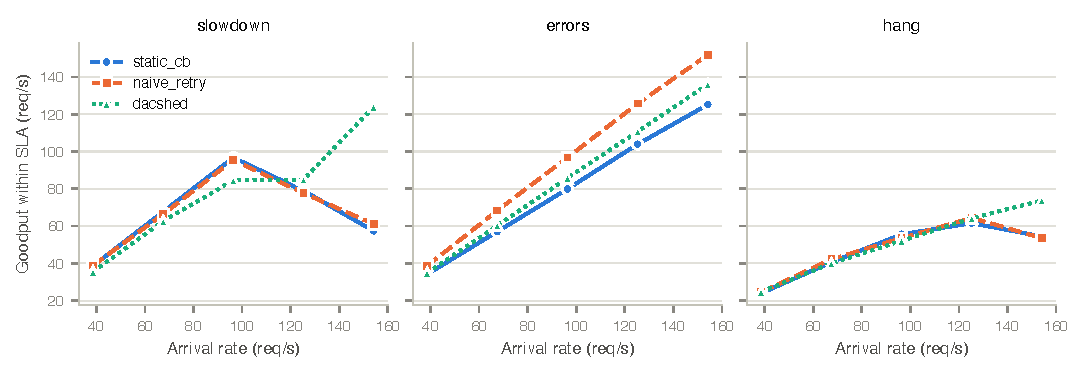
\includegraphics[width=\textwidth]{fig08.pdf}
  \caption{Goodput within the 250\,ms SLA against offered rate for each injected fault, with one panel per fault and one series per controller. Each point averages two runs.}
  \label{fig:goodput}
\end{figure*}

\paragraph{Replicate spread.} Across the 45 cells of Phase~5, the median gap in goodput between the two replicates of a cell is $1.19$\,req/s, and the mean gap is $2.61$\,req/s. At the highest load the median gap is $1.35$\,req/s, and the largest gap is $8.39$\,req/s, for the naive retry under the hang. DAC-Shed varies by $0.01$\,req/s under errors and by $0.69$\,req/s under the hang at that load. The advantage of DAC-Shed at the highest load, $+62.9$\,req/s over the naive retry under slowdown ($124.0$ against $61.1$), is larger than the largest replicate gap of the two compared cells, $7.95$\,req/s. Its advantage under the hang, $+20.3$\,req/s over the naive retry ($73.7$ against $53.5$), is larger than the $8.39$\,req/s gap of that cell. At the request level ($N \approx 24{,}670$ measured requests pooled across the two $80\text{ s}$ post-warmup windows at $154.2\text{ req/s}$), the 95\% binomial bootstrap confidence interval half-width on goodput is at most $\pm 1.54\text{ req/s}$ across all 45 cells ($\pm 1.22\text{ req/s}$ for DAC-Shed under slowdown and $\pm 1.53\text{ req/s}$ under hang), confirming that both within-run sampling uncertainty and between-replicate spread are an order of magnitude smaller than the controller separation.

\paragraph{Offline replay of a budget-gated retry.} The retry that the error results suggest is worth testing, so we replayed it offline on the stored Phase~5 traces. The replay is a counterfactual on recorded data, not a live experiment, and it was designed after the Phase~5 results were known. A single retry is permitted only when the first attempt returned an injected error, when the remaining budget satisfies $B_{\mathrm{rem}}\ge 2\cdot\mathrm{floor}(v)$, and when the latency gradient is below $3.0$. The replayed attempt draws its latency from the empirical distribution of successful calls in the same run.

On the two replicates at 154.2\,req/s, the replay recovers $69.3\%$ and $69.0\%$ of first-attempt errors within the 250\,ms SLA, which is $69.2\%$ pooled. The goodput of DAC-Shed rises from $136.0$\,req/s, with a success fraction of $0.89$, to $147.4$\,req/s, with a success fraction of $0.97$. That is close to the $151.8$\,req/s of naive retries, and the replay adds $2.7\%$ extra hop invocations. Under the slowdown and hang faults, the gate blocks 100\% of retries through both mechanisms simultaneously: failed requests time out or are shed rather than returning a transient callee error code, and stored hop telemetry confirms that local queueing drives the Vegas latency gradient above the $\gamma_v \ge 3.0$ threshold while exhausting $B_{\text{rem}} < 2\cdot\text{floor}(v)$. Consequently, replaying the gate across the slowdown and hang traces triggers zero retries and preserves DAC-Shed's exact $124.0\text{ req/s}$ and $73.7\text{ req/s}$ goodput curves. Because this evaluation is an offline trace-replay counterfactual assuming independent retry draws and negligible queueing perturbation from the $2.7\%$ additional hop calls, live closed-loop evaluation under bursty multi-hop faults is noted as a direction for future work.
